%% =====================================================================
\section{Related work}
\label{sec:related_work}
%% =====================================================================

%% Related work is reviewed by problem type, without a ``four-layer positioning''. Older literature is kept as citation clusters; the narrative focuses on recent work.

A basic question in dynamic scheduling is on which object the rescheduling scope is delineated after a disturbance, that is, what is changed and what is kept as planned.
The literature delineates this scope on different objects: operations or the time axis, the occupancy order on exclusive resources,
the affected vehicles, and the set of operations in the flexible job shop with transportation.
We review, for each of these four classes, what has been done and what remains uncovered, and summarize them in Table~\ref{tab:position}.

\subsection{Local rescheduling in job shops}
\label{sec:rw_aor}

For operation-level events such as machine breakdowns and rush-order insertions, delineating the rescheduling scope by the affected operations is still common in dynamic scheduling with AGVs.
Zhang et al.~\cite{zhang2023energy} handle machine breakdowns and rush orders, taking as the recovery scope the operations not yet processed after the breakdown.
Tang et al.~\cite{tang2026dynamic} classify operations and delivery tasks, according to the impact of the disturbance, as retained, continued, or reconstructed.
They compare full rescheduling, partial rescheduling, and right shift side by side, noting that right shift preserves stability at the cost of optimization room.
The original sentences underlying the paraphrases used for positioning in this and the next subsection are listed in Table~\ref{tab:refcheck}.
This practice dates back to affected-operation rescheduling (AOR)~\cite{abumaizar1997rescheduling,subramaniam2003maor},
which reschedules only the operations directly or indirectly affected by the disturbance.
Delineating the scope along the time axis and enlarging it after failure have also been studied, including match-up~\cite{akturk1999matchup}
and Local Rescheduling with incrementally enlarged time windows~\cite{kuster2007local}.
Right shift, in contrast, does not determine which operations are affected; it postpones the entire unfinished part.
Rolling-horizon and decomposition methods trade off scale against quality~\cite{zeitrag2025novel,zhao2019decomposition};
see~\cite{vieira2003rescheduling,ouelhadj2009survey} for surveys.

These works show that delineating a scope and then rescheduling locally is not a new problem, provided that the disturbance acts on operations in the first place.
Once a disturbance only makes a corridor impassable without changing any assignment, the scope delineated by this approach can be empty, even though the original schedule is already infeasible.

\subsection{Occupancy order on exclusive resources}
\label{sec:rw_ag}

Modeling ``who occupies the same exclusive resource first'' as a graph has been studied systematically in railway scheduling.
The alternative graph of Mascis and Pacciarelli~\cite{mascis2002alternative}
generalizes the disjunctive graph: vertices are occupations of block sections by operations, fixed arcs encode route precedence,
and paired alternative arcs encode which train passes the section first.
D'Ariano et al.~\cite{dariano2007branch} use this model for real-time train rescheduling,
recomputing a conflict-free timetable after a disturbance while staying as close as possible to the original plan.
Yielding relations on the same corridor express the same kind of precedence as alternative arcs.

The difference from this paper lies in how the precedence is used. For each conflict, the alternative graph provides two mutually exclusive arcs
(A passes first, or B passes first), and scheduling amounts to selecting one of them.
The timetable is feasible only if the selection leaves no positive-weight cycle, and the objective is optimized as far as possible; occupancy order is therefore a decision variable.
In this paper the plan has already been scheduled, and who passes which corridor first is already fixed. We do not choose the order again;
we only use these established yielding and succession relations to bring the original corridor occupancies invalidated by the disturbance into the rescheduling scope.
Moreover, the railway model treats block sections as machines, so operations and occupancies live on the same graph,
and an unavailable section is itself an operation-level event. Hence the problem of ``a scope delineated on the operation-precedence graph missing a corridor blockage'' does not arise there.
In the flexible job shop, processing and corridor occupancy are two separate sets of objects, and existing AOR scoping does not exploit the occupancy order.

\subsection{Local replanning in conflict-free multi-vehicle routing}
\label{sec:rw_mapf}

In multi-agent path finding (MAPF), replanning only the affected agents while treating the others as dynamic obstacles is standard practice.
For online MAPF, \v{S}vancara et al.~\cite{svancara2019online} propose
% selfcheck:allow-term ``affected set'' here denotes the output of MAPF independence detection, not the name of our mechanism
Replan All, Replan Single, and Replan Affected, and determine the affected set by online independence detection.
Malka et al.~\cite{malka2024online} likewise replan only the vehicles affected by observed changes when the map is inaccurate.
% selfcheck:allow-term ``spatiotemporal occupancy'' is an established MAPF term; here it paraphrases the cited work and does not refer to our corridor occupancy
Conflict-free path planning treats spatiotemporal occupancy as a first-class constraint, but start and goal locations are usually given externally~\cite{zhang2024guidance}.

These works have already made ``change only the affected, keep the rest as planned'' a standard mechanism, which we adopt.
They differ from our setting in that they have only vehicle start and goal locations and no job--operation--machine assignment.
Hence the situation in which ``the rescheduling scope is delineated on the operation-precedence graph and a corridor blockage is missed for lack of an affected operation'' cannot arise.
% selfcheck:allow-term ``affected set'' is a neutral term shared by both approaches here; the second half of the sentence states that it is the output of a detection algorithm
As for how the affected set is obtained, MAPF finds the affected vehicles by independence detection; the result is the output of a detection algorithm and varies with its implementation and stopping condition.
The reservation impact set proposed here differs: once the dependency edges are given, whether an occupancy belongs to the set
depends only on whether it is reachable from the seeds along these edges, independently of the rerouting algorithm used afterwards
(Section~\ref{sec:containment}).

\subsection{Flexible job shop scheduling with transportation}
\label{sec:rw_position}

Flexible job shop scheduling with transport vehicles has been systematically surveyed~\cite{xin2025review}.
Recent combinatorial optimization work still commonly takes travel times as a constant matrix indexed by location pairs,
and builds constraint programming, metaheuristics, and knowledge-guided search on top of it~\cite{meng2025cp,qin2026knowledge,fu2025integrated}.
Under this convention vehicles do not compete for the same road segment, so a corridor blockage has no counterpart in the model and cannot be tested.

Once corridor occupancies are recorded as time windows, both processing order and corridor occupancy enter the model.
Congestion-aware dispatching can select vehicles using proxies such as local density, without changing machine assignments~\cite{kim2026congestion}.
Work that jointly models flexible assignment and conflict-free transportation is relatively scarce.
Van Os and Basten~\cite{vanos2026exact} formalize flexible job shop scheduling with conflict-free transportation constraints
and, with a decomposition method, obtain provably optimal solutions on most benchmark instances; for a few, optimality cannot be guaranteed because of the time limit.
Two-stage schemes first fix the production schedule and then resolve vehicle conflicts~\cite{sun2023integrated}.
There is also a framework with a learning-based scheduling layer and a conflict-resolving routing layer, connected by limited feedback~\cite{li2026framework}.
These works, however, address how to build a feasible, high-quality conflict-free schedule before execution starts.

Among the works cited in this section, a corridor reservation table and a response to execution-time disturbances never appear together: works with a reservation table exclude execution-time failures,
and works that handle execution-time disturbances have no reservation table.
For example (original sentences in Table~\ref{tab:refcheck}),
Zhang et al.~\cite{zhang2023energy} state in their modeling assumptions that collisions between AGVs are ignored.
Sun et al.~\cite{sun2023integrated}
resolve vehicle conflicts with a time-window Dijkstra algorithm, yet assume that vehicle charging and failures are not considered and that vehicles are always available;
they list equipment maintenance and breakdowns as future research.

The gap therefore arises because two conditions have not been met together.
Operation-level scoping is often valid precisely because the model contains no corridor reservations, while settings with a reservation table exclude execution-time disturbances.
When both are present, the only directly applicable practice is scoping by affected operations,
which yields an empty scope for a corridor blockage that does not change any operation assignment (measured in Section~\ref{sec:e1}: \PassMiss).
This is exactly the situation addressed in this paper.

\begin{table}[t]
\centering
\caption{The five paraphrases on which we base the gap, with the cited original text (English sentences quoted verbatim).}
\label{tab:refcheck}
\footnotesize
\begin{tabular}{@{}p{0.23\linewidth}p{0.55\linewidth}p{0.14\linewidth}@{}}
\toprule
\textbf{Our paraphrase} & \textbf{Cited original text} & \textbf{Location in source} \\
\midrule
Zhang et al.~\cite{zhang2023energy} take as the recovery scope the operations not yet processed after the breakdown &
\emph{``Rearrange the unprocessed operations of current scheme considering the limit of
machine breakdown''} &
Rescheduling procedure \\
\addlinespace
Zhang et al.~\cite{zhang2023energy} state in their modeling assumptions that collisions between AGVs are ignored &
\emph{``The collision of AGVs are ignored.''} &
Modeling assumption (7) \\
\addlinespace
Tang et al.~\cite{tang2026dynamic} classify operations and delivery tasks by disturbance impact as retained, continued, or reconstructed &
\emph{``an event-driven partial rescheduling strategy is proposed, in which the disrupted
operations and delivery tasks are classified into three categories: retained, continued,
and reconstructed''} &
Abstract \\
\addlinespace
Van Os and Basten~\cite{vanos2026exact} obtain provable optimality on most benchmark instances;
for a few, optimality cannot be guaranteed because of the time limit &
\emph{``For most benchmark instances, our LBBD-based approach finds optimal makespan
values. Because of time boxing, only in a few cases, the optimality of the found solution
cannot be guaranteed.''} &
Abstract \\
\addlinespace
Sun et al.~\cite{sun2023integrated} assume vehicles are always available, ignore failures and charging,
and list equipment maintenance and breakdowns as future research &
\emph{``It does not consider the charging problem and fault problem of the AGVs, and AGVs
are always available''}; \emph{``Breakdowns and charging problems are not taken into
account.''}; \emph{``Future research will investigate the impact of equipment maintenance
and breakdowns on production scheduling''} &
Assumption list; future work \\
\bottomrule
\end{tabular}
\end{table}

\subsection{Positioning of this paper}
\label{sec:rw_claim}

\begin{table*}[t]
\centering
\caption{Related work classified by \emph{scope object}: the kind of object on which each class defines ``what must be rewritten'' after a disturbance.
``Scope delineated on'' is the object to which the rescheduling scope is attached; ``Operation-precedence graph?'' also indicates whether that graph coincides with the occupancy graph.
The bold entry in the last row marks the class to which this paper belongs.}
\label{tab:position}
\small
\begin{tabular}{@{}p{0.16\linewidth}p{0.22\linewidth}p{0.14\linewidth}p{0.14\linewidth}p{0.24\linewidth}@{}}
\toprule
\textbf{Class} & \textbf{Representative work} & \textbf{Scope delineated on} & \textbf{Operation-precedence graph?} & \textbf{Relation to this paper} \\
\midrule
Local rescheduling in job shops &
AOR~\cite{abumaizar1997rescheduling,subramaniam2003maor};
match-up~\cite{akturk1999matchup};
LRS~\cite{kuster2007local};
dynamic scheduling with AGVs~\cite{zhang2023energy,tang2026dynamic} &
Operations / time windows & Yes &
Operation-level scoping and right shift are reproduced as baselines later \\
\addlinespace[2pt]
Occupancy order on exclusive resources &
alternative graph~\cite{mascis2002alternative};
real-time railway rescheduling~\cite{dariano2007branch} &
Block-section occupancies & Yes, on the same graph as occupancies &
Same kind as yielding relations; railways use it to choose the order of trains, whereas we use the established order to delineate the occupancies that must be rewritten \\
\addlinespace[2pt]
Conflict-free multi-vehicle routing &
Online MAPF~\cite{svancara2019online,malka2024online};
LMAPF~\cite{zhang2024guidance} &
Affected vehicles & No &
Rerouting inside the set and keeping the rest as planned is already standard \\
\addlinespace[2pt]
Flexible job shop with transportation &
constant matrix~\cite{xin2025review,meng2025cp,qin2026knowledge,fu2025integrated};
integrated scheduling~\cite{vanos2026exact,sun2023integrated,li2026framework} &
Set of operations & Yes; reservation table and execution-time disturbances never appear together &
\textbf{Position of this paper} \\
\bottomrule
\end{tabular}
\end{table*}

In summary, in the flexible job shop with conflict-free AGV routing, a schedule uses operation precedence to describe processing order
and time windows to record corridor occupancy. This gives rise to the situation corresponding to the gap identified above:
a disturbance such as a corridor blockage does not make any operation inexecutable, and the original assignment remains valid,
yet the corridor occupancies overlapping the disturbed interval are invalidated, so the original schedule is infeasible.
The baseline that scopes on the operation-precedence graph later in the paper reproduces the practice of Section~\ref{sec:rw_aor}.
We propose moving the rescheduling scope onto corridor occupancies and their yielding and succession relations, which yields a reservation impact set uniquely determined by these relations.

%% =====================================================================
\section{The corridor-reservation setting and the execution-time recovery problem}
\label{sec:problem}
%% =====================================================================

\subsection{System setting and notation}
\label{sec:system_brief}

The problem setting follows the flexible job shop with conflict-free transportation constraints~\cite{vanos2026exact}.
This subsection defines, once and for all, the objects used later. A feasible schedule \(\mathcal{S}^0\) is taken as a given input:
how it was found at \(t=0\) does not affect how we later delineate the occupancies that must be rewritten.

\subsubsection{Shop floor and four groups of decisions}
\label{sec:shop}

The shop routing graph \(G=(V,E)\) is strongly connected. Each machine \(m\) performs processing through a robotic arm located at a fixed node \(\mathrm{loc}(m)\);
a robotic-arm failure below means the failure of that machine.
\(v_0\in V\) is the load/unload station. There are \(n\) jobs, a machine set \(M\), and a homogeneous fleet of unit-load vehicles
\(K=\{1,\ldots,N_A\}\). Job \(j\) has a fixed chain of operations \(O_{j1}\to\cdots\to O_{jn_j}\);
operation \(O_{ji}\) has a candidate machine set \(\Omega_{ji}\subseteq M\) and processing time
\(t^P_{jim}\) on machine \(m\). A complete schedule fixes four groups of decisions simultaneously:
(i)~the machine assignment \(x\) of each operation;
(ii)~the processing sequence \(\pi\) of operations on each machine;
(iii)~the vehicle assignment \(y\) of each transport;
(iv)~a conflict-free path on \(G\) for each vehicle move.
We write
\[
\mathcal{S}=(x,\,\pi,\,y,\,R),
\]
where the reservation table \(R\) is the explicit record of group (iv), defined below.

Transport tasks are \emph{derived} from the assignment rather than given as input: a transport arises only when two consecutive operations are at different nodes.
Each transport is split into two legs, an empty leg for pickup and a loaded leg for delivery, each with its own task label \(u\)
(for example, the empty leg and the loaded leg of \(O_{ji}\) are two separate records). Loading and unloading times are zero: the loaded leg departs at the later of
the empty leg's arrival and the job's ready time, and the delivery time is simultaneously the time at which the machine can start and the vehicle can accept a new task.
Which occupancies are rewritable, which are kept as planned, and how rerouting is done are all decided at the granularity of legs, not whole operations.

\subsubsection{Corridor reservation and conflict freedom}
\label{sec:reservation}

Each corridor \(e\in E\) is an exclusive resource with known traversal time \(\tau_e\). Both directions share the same occupancy,
so at most one vehicle occupies \(e\) at any time, which rules out both head-on conflicts and same-direction overtaking.
Occupancies are half-open intervals: a second vehicle may enter exactly at the right endpoint of the interval.
Nodes have ample parking capacity, so waiting takes place at nodes and is always allowed.
A reservation record is
\[
r=(e,\,[t^s,t^e),\,k,\,u)\in R,
\]
meaning that vehicle \(k\) occupies corridor \(e\) during \([t^s,t^e)\) for leg \(u\).
Any two distinct occupancies of the same corridor must satisfy
\([t^s,t^e)\cap[t^{s\prime},t^{e\prime})=\varnothing\).
Paths are written only into time windows that \(R\) reports as free, so conflict freedom holds by construction.

Time-window routing is the primitive shared by our rerouting and by all baseline methods: given the origin and destination, the earliest departure time, and the current \(R\),
it returns a path disjoint from existing occupancies together with the entry time of each corridor.
We implement it as a time-window Dijkstra algorithm~\cite{sun2023integrated}. We do not modify this primitive;
we change only \emph{which} transport legs are sent to the router.
Unlike van Os, who reserves nodes, and Lyu, who additionally imposes node capacities~\cite{vanos2026exact,lyu2019approach},
we reserve edges; Section~\ref{sec:limitations} discusses the resulting restrictions on instance scope.

\subsubsection{Operation-precedence graph and reservation dependency graph}
\label{sec:two_graphs}

% selfcheck:allow-term ``task graph'' is a synonym retained by ruling B13, and also explains the subscript of \(G_T\)
The operation-precedence graph \(G_T=(T_T,E_T)\) (also called the task graph in the literature; the subscript \(T\) stands for task) has operations as vertices
and job precedence and same-machine precedence as edges;
it does \emph{not} contain the yielding relations between corridor occupancies.
The reservation dependency graph \(G_R=(R,E_R)\) has the occupancies in \(R\) as vertices, and its edges are the dependencies induced by yielding, same vehicle, same job, and same machine
(Definition~\ref{def:dep}).
The vertex sets of the two graphs are disjoint: one represents processing, the other traversal.
Hence there is a class of disturbances that changes only corridor time windows and no operation parameter. Scoping on \(G_T\) finds no seed operation,
whereas scoping on \(G_R\) yields a nonempty seed set, and the original schedule is already infeasible.
Figure~\ref{fig:graphs} contrasts the two graphs, Figure~\ref{fig:motivate} shows the consequences under a corridor blockage, and
Table~\ref{tab:notation} summarizes the notation used in this section and later.

\begin{figure}[t]
\centering
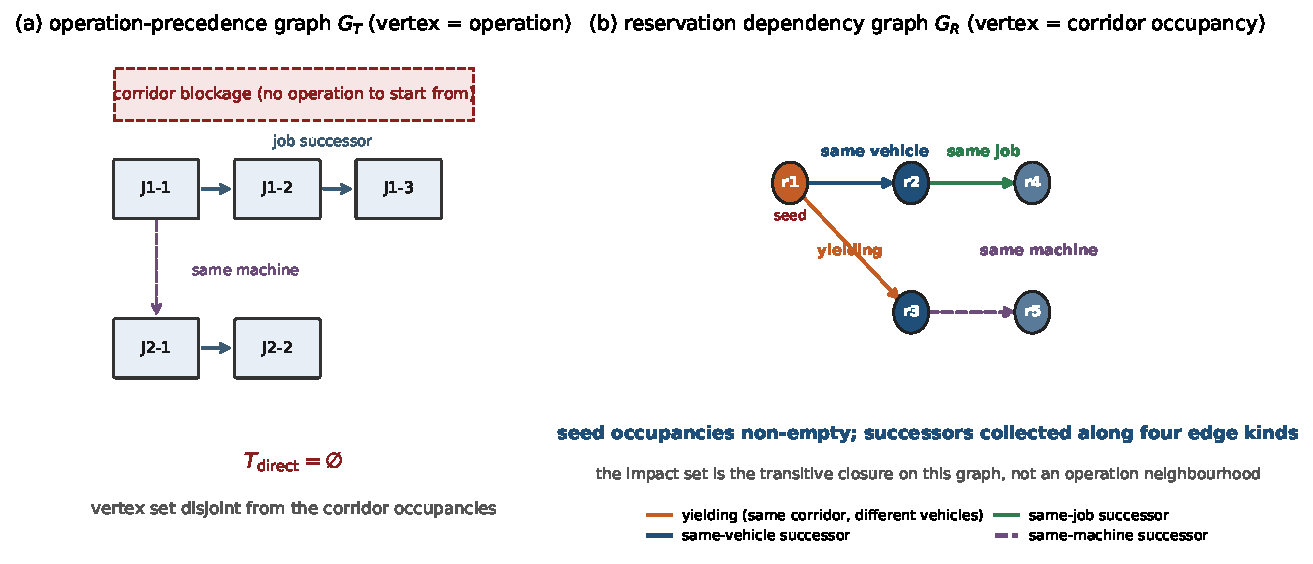
\includegraphics[width=\linewidth]{figures/fig_strc_graphs}
\caption{The vertex sets of the two graphs are disjoint (schematic construction).
(a)~Operation-precedence graph \(G_T\): vertices are operations, and a corridor blockage finds no seed operation.
(b)~Reservation dependency graph \(G_R\): vertices are corridor occupancies; starting from the occupancies overlapping the blockage window, subsequent occupancies are included along the four kinds of dependency edges
(yielding, same vehicle, same job, same machine; Definition~\ref{def:dep}).}
\Description{Two panels side by side. The left panel is the operation-precedence graph, with job-successor and same-machine-successor edges connecting operation boxes;
a dashed box at the top marks the corridor blockage, which does not fall on any box.
The right panel is the reservation dependency graph, with five circular vertices representing corridor occupancies and arrows in four colors labeled
yielding, same vehicle, same job, and same machine.}
\label{fig:graphs}
\end{figure}

\begin{table}[t]
\centering
\caption{Frequently used notation}
\label{tab:notation}
\small
\begin{tabular}{@{}ll@{}}
\toprule
\textbf{Symbol} & \textbf{Meaning} \\
\midrule
\(G=(V,E)\), \(\tau_e\) & Corridor network; traversal time of corridor \(e\) \\
\(v_0\), \(\mathrm{loc}(m)\) & Load/unload station; node of robotic arm \(m\) \\
\(x,\pi,y\) & Machine assignment, processing sequence, vehicle assignment \\
\(R\), \(r=(e,[t^s,t^e),k,u)\) & Reservation table; a half-open occupancy (vehicle \(k\), leg label \(u\))\\
\(G_T\) / \(G_R\) & Operation-precedence graph / reservation dependency graph \\
\(\mathcal{S}^0,\mathcal{S}'\) & Schedule before the disturbance, schedule after recovery \\
\(\mathcal{D},\,t_{\mathrm{now}}\) & Disturbance event; occurrence (decision) time \\
\(T_{\mathrm{direct}},\,T_{\mathrm{impact}}\) & Directly disturbed operations on the operation-precedence graph / \(\theta\)-step scope \\
\(\mathrm{Src}(\mathcal{D})\), \(U\) & Seed occupancies; set of rewritable occupancies \\
\(\mathrm{Cl}(\cdot)\) & Reservation impact set (obtained by \STRC)\\
\(\varphi\) & Fraction of disturbed future operations (magnitude sweep)\\
\bottomrule
\end{tabular}
\end{table}

\subsection{Execution-time assumptions}
\label{sec:assumptions}

The execution-time conventions and physical setting are as follows. A1--A4 are shared by all compared methods, so that differences in results can be attributed to how the rescheduling scope
is delineated rather than to model differences. A5 constrains only our method; the global-rescheduling baseline is allowed a wider set of actions (see the last sentence of A5):

\begin{enumerate}[label=\textbf{A\arabic*.},leftmargin=*,topsep=2pt,itemsep=2pt]
\item \textbf{Feasible initial schedule.} \(\mathcal{S}^0\) passes the conflict-freedom check before the disturbance, and the reservation table is consistent with the operation timetable.
\item \textbf{No backtracking on finished occupancies.} Only unfinished occupancies with \(t^e>t_{\mathrm{now}}\)
and unfinished operations are rewritten; the fields of occupancies with \(t^e\le t_{\mathrm{now}}\) are not rewritable.
\item \textbf{Single, fully observed disturbance.} The disturbance is fully observed at \(t_{\mathrm{now}}\) and does not overlap with other disturbances;
disturbance streams, prediction errors, and rolling responses are beyond the scope of this paper.
\item \textbf{Exclusive corridors, ample buffers, homogeneous unit-load fleet.} Corridors remain exclusive half-open resources, and a blockage is injected into the routing layer as an additional occupancy
(or forbidden window). Finite buffers, charging, acceleration and deceleration, and loading/unloading durations are not modeled;
all vehicles start empty at \(v_0\) at the beginning of the plan.
\item \textbf{Permitted recovery actions.} For Class B disturbances, the original machine assignment \(x\) and processing sequence \(\pi\) are kept and only rerouting is performed;
upon failure, the set of rewritable occupancies is escalated. Class A failures additionally allow the following: a vehicle failure removes the failed vehicle from the fleet and reassigns its tasks to another vehicle;
a robotic-arm failure reassigns unfinished operations to other feasible machines. The processing sequence \(\pi\) is never changed, and the search is not restarted.
The global-rescheduling baseline in the experiments may change \(x\) and \(\pi\) (Section~\ref{sec:vs_r0}).
\end{enumerate}

\subsection{A dichotomy of disturbances}
\label{sec:disturbance_classes}

\begin{definition}[Class A/B disturbances]
\label{def:ab}
A disturbance is of \textbf{Class A} if it directly invalidates the assignment or \emph{executability} of some operations (robotic-arm failure, significant processing-time deviation, rush-order insertion,
vehicle failure, etc.). It is of \textbf{Class B} if it only makes some corridor time windows unavailable without making any operation
inexecutable (corridor blockage, corridor slowdown, etc.).
\end{definition}

\begin{remark}[Why vehicle failure is Class A]
\label{rem:agv_class}
A vehicle failure does not change the machine assignment of any operation, so at first sight it seems to belong with corridor blockages. However, the criterion in Definition~\ref{def:ab} is
\emph{executability}, not assignment: after a vehicle fails, the operations it transports cannot start under the original plan.
Through the mapping ``vehicle\(\to\)operations it transports'', the operation-precedence graph therefore still contains seed operations. This classification places vehicle failure
on the side where operation-level scoping gives a nonempty scope.
These seed operations are nonempty only if the rescheduling method maintains a vehicle--task mapping; if the method tracks only operations and machines
(as common AOR implementations do), a vehicle failure also yields an empty scope.
Section~\ref{sec:e6} reports Class A results under the convention that this mapping is maintained.
\end{remark}

\begin{definition}[Direct set and affected set on the operation-precedence graph]
\label{def:task_impact}
For a disturbance \(\mathcal{D}\), let \(T_{\mathrm{direct}}(\mathcal{D})\) be the set of operations that cannot be executed as planned because of a robotic-arm failure, a vehicle failure, or operation invalidation.
For Class B corridor disturbances, we set \(T_{\mathrm{direct}}=\varnothing\) by convention.
Starting from \(T_{\mathrm{direct}}\) on \(G_T\), the operations reached along job-successor and same-machine-successor edges within depth at most \(\theta\) form
\(T_{\mathrm{impact}}(\mathcal{D},\theta)\).
\end{definition}

\begin{definition}[Seed occupancies]
\label{def:seeds}
The seed set \(\mathrm{Src}(\mathcal{D})\subseteq R\) is given by disturbance type and always includes only occupancies with
\(r.t^e>t_{\mathrm{now}}\).
\begin{enumerate}[label=(\alph*),leftmargin=1.6em,itemsep=0.15em]
\item \textbf{Corridor blockage/slowdown} \(\mathcal{D}=(e,[t_a,t_b))\):
\(\{\,r:\ r.e=e,\ [r.t^s,r.t^e)\cap[t_a,t_b)\neq\varnothing\,\}\).
For multiple short blockages, the union of the seed occupancies of all windows is taken. Blockage and slowdown share this seed rule (the original schedule was written with the unscaled \(\tau\),
so every occupancy overlapping the window is invalidated); hence they yield the same reservation impact set when delineating the occupancies to be rewritten. Section~\ref{sec:e6} uses this to explain
why their scoping results are not counted as two independent validations. They differ in rerouting: a blockage is written as a forbidden window,
whereas a slowdown only scales, by a factor, the traversal progress in the part overlapping the window.
\item \textbf{Vehicle failure} \(\mathcal{D}=(k)\): all occupancies of that vehicle after \(t_{\mathrm{now}}\),
\(\{\,r:\ r.k=k\,\}\).
\item \textbf{Robotic-arm failure} \(\mathcal{D}=(m,F)\), where \(F\) is the set of unfinished operations on that machine:
for each job, take the smallest operation index \(i_{\min}(j)\) in \(F\); the seed occupancies are all unfinished occupancies of each job from that operation onward (inclusive).
We take the job chain forward rather than only the operation itself because its inbound transport may have finished before
\(t_{\mathrm{now}}\); taking only the operation itself would make the reservation impact set shorter than the affected set on the operation-precedence graph, and the comparison would be unfair.
\end{enumerate}
\end{definition}

\begin{prop}[The operation-precedence graph yields an empty scope for Class B]
\label{prop:miss}
Let \(\mathcal{D}\) be a corridor blockage. Under the Class B convention of Definition~\ref{def:task_impact},
\(T_{\mathrm{direct}}(\mathcal{D})=\varnothing\), and hence \(T_{\mathrm{impact}}(\mathcal{D},\theta)=\varnothing\) for every finite \(\theta\ge 0\).
If, in addition, \(\mathrm{Src}(\mathcal{D})\neq\varnothing\), then \(\mathcal{S}^0\) is infeasible under \(\mathcal{D}\).
\end{prop}

\begin{proof}
A corridor blockage only makes corridor time windows unavailable without making any operation inexecutable, so it is of Class B by Definition~\ref{def:ab}.
This step relies on two premises: the blockage window \([t_a,t_b)\) is finite, and by Assumption A4 buffers are ample, so vehicles can traverse outside the window.
Hence, even if the network is disconnected during the blockage, no operation becomes inexecutable; operations are only delayed. If the blockage were indefinite,
or buffers were insufficient to support waiting, the disturbance would be of Class A by Definition~\ref{def:ab} and would fall outside the scope of this proposition.
Being of Class B,
it has \(T_{\mathrm{direct}}=\varnothing\) by the Class B convention of Definition~\ref{def:task_impact}.
The starting set of the \(\theta\)-step expansion is empty, so \(T_{\mathrm{impact}}=\varnothing\).
If some \(r\in\mathrm{Src}(\mathcal{D})\) exists, the occupancy interval of \(r\) intersects the forbidden window.
Interpreting \(\mathcal{D}\) as a mandatory occupancy of that corridor, \(r\) and the forbidden window overlap in time on the same exclusive resource,
which violates the half-open time-window conflict-freedom condition (corridor exclusivity in Assumption A4). Hence \(\mathcal{S}^0\) is infeasible.
\end{proof}

Proposition~\ref{prop:miss} is a counterexample at the problem level. Its first part follows directly from the Class B convention of Definition~\ref{def:task_impact}
(by definition, the operation-precedence graph does not contain the yielding relations between corridor occupancies and thus cannot represent a corridor blockage).
The nontrivial part is the second: when the seed set is nonempty, the original schedule is already infeasible.
Hence ``an empty scope on the operation-precedence graph \(\Rightarrow\) no rescheduling needed'' does not hold in a setting where corridors are reserved by time windows.
The counterexample does not depend on any repair algorithm; Section~\ref{sec:experiments} reports its extent on the instances.

\subsection{The recovery problem}
\label{sec:recovery_problem}

\begin{problem}[Bounded repair with the scope delineated on the reservation table]
\label{prob:recovery}
Given a feasible schedule \(\mathcal{S}^0\), a disturbance \(\mathcal{D}\), and a time \(t_{\mathrm{now}}\),
find \(\mathcal{S}'\) such that
(i)~\(\mathcal{S}'\) passes the conflict-freedom check under \(\mathcal{D}\);
(ii)~occupancies outside the rewrite scope keep their corridors, time intervals, and vehicles as close to \(\mathcal{S}^0\) as possible;
(iii)~the runtime is subject to a budget.
The secondary objective is the makespan \(C_{\max}(\mathcal{S}')\).
\end{problem}

The solution proceeds in two steps: first delineate the set of rewritable occupancies \(U\subseteq R\);
then reroute only the transports in \(U\), keeping occupancies outside the set as planned.
We obtain \(U\) as \(\mathrm{Cl}(\mathrm{Src})\); the baselines instead derive a reservation subset from the affected set on the operation-precedence graph.

%% =====================================================================
